\documentclass{article}

% if you need to pass options to natbib, use, e.g.:
%     \PassOptionsToPackage{numbers, compress}{natbib}
% before loading neurips_2019

% ready for submission
% \usepackage{neurips_2019}

% to compile a preprint version, e.g., for submission to arXiv, add add the
% [preprint] option:
%     \usepackage[preprint]{neurips_2019}

% to compile a camera-ready version, add the [final] option, e.g.:
\usepackage[final]{neurips_2019}

% to avoid loading the natbib package, add option nonatbib:
%     \usepackage[nonatbib]{neurips_2019}

\usepackage[utf8]{inputenc} % allow utf-8 input
\usepackage[T1]{fontenc}    % use 8-bit T1 fonts
\usepackage{hyperref}       % hyperlinks
\usepackage{url}            % simple URL typesetting
\usepackage{booktabs}       % professional-quality tables
\usepackage{amsfonts}       % blackboard math symbols
\usepackage{nicefrac}       % compact symbols for 1/2, etc.
\usepackage{microtype}      % microtypography
\usepackage{amsmath}
\usepackage{xcolor}
\usepackage{amssymb}
\usepackage{graphicx}
\usepackage{float}
\usepackage{graphicx}
\usepackage{multirow}
\usepackage{natbib} 
\graphicspath{ {./imgs/} }


\title{Dynamic Training Planning to Boost the Performance of Deep Neural Network (DNN)}

% The \author macro works with any number of authors. There are two commands
% used to separate the names and addresses of multiple authors: \And and \AND.
%
% Using \And between authors leaves it to LaTeX to determine where to break the
% lines. Using \AND forces a line break at that point. So, if LaTeX puts 3 of 4
% authors names on the first line, and the last on the second line, try using
% \AND instead of \And before the third author name.

\author{
  Ramesh Sankaranarayana \\
  College of Engineering \& Computer Science \\
  the Australian National University\\
  Canberra ACT 2600 Australia\\
  \texttt{ramesh@cs.anu.edu.au} \\
  \And
  Limin Deng\\
  College of Engineering \& Computer Science \\
  the Australian National University\\
  Canberra ACT 2600 Australia\\
  \texttt{u6849956@anu.edu.au} \\
}

\begin{document}

\maketitle

\begin{abstract}

This paper is focused on training planning, which specifically refers to data preprocessing, training strategy, and post processing, to boost the performance of deep neural network (DNN). DNN has made a lot of success in many applications, such as classification and segmentation, and efficient training planning is essential to boost the performance of models. For example, in the Prostate cANcer graDe Assessment (PANDA) Challenge, the data are whole-slide images (WSI), which have dramatically diverse image size (from 1000 to 14000 pixels in the middle resolution) and pixel intensities (from 735000 to 29420000 pixels). To solve this problem, we utilized a series of dynamic methods, such as dynamic switch level, bin threshold, and dynamic tiling to maximally extract features. Our approaches achieved a quadratic weighted kappa of 0.92096 on the private leaderboard of PANDA challenge. It can rank 50 out of 1010 teams according to the finalized private leaderboard. We found our post processing approach can boost the model performance by around 0.3. The code is freely available at https://github.com/muerbingsha/kaggle-panda-paper.   \par

\textbf{Keywords:} Prostate cancer(PCa), Gleason grading, whole-slide images(WSI), dynamic tiling


\end{abstract}





\section{Introduction}

Image classification and segmentation have wide applications, such as in Deepfake detection \citep{bonettini2020video}, diabetic classification \citep{mateen2020exudate}, and prostate cancer classification \citep{duran2020prometeo}. Currently, the main stream is to use deep neural network (DNN) to study classification and segmentation problems. To date, most studies have utilized U-Net \citep{ronneberger2015u}, Resnet \citep{he2016deep}, Efficientnet \citep{tan2019efficientnet},  Densenet \citep{huang2017densely}, Inception V3 \citep{szegedy2016rethinking}. My task is mainly focused on data preprocessing, training strategy, and post processing, which are significant to improve the performance of models. One important work in Kaggle competiton is on training planning, to map the features of seen training data set to unseen test set. Due to the leaderboard of Deepfake detection has closed after the competition, I don't have an official metric to evaluate performance while the leaderboard of Prostate cANcer graDe Assessment (PANDA) Challenge remains open. Thus, I put energy on the PANDA competition to test my ideas.

The workflow of diagnosing prostate cancer (PCa) is as follows: a prostate biopsy is needed when the initial tests, such as prostate-specific antigen (PSA) blood test or digital rectal exam, return alert results (Prostate biopsy - Mayo Clinic, 2020). Pathologists get the tissue samples, stain with hematoxylin and eosin (H\&E), and scan into whole-slide images(WSI) to review on computer. The severity of PCa is graded by Gleason score which can be converted into the International Society of Urological Pathology (ISUP) grade on a 0-5 scale. This process is time-consuming and error-prone since WSI is a pyramid of data and has very large resolutions (up to 14000 pixels in middle resolution). Besides, WSI has variant image quality such as various H\&E stain color, pen marks (red, blue, green), and artifacts in blur, bad sample slice and scan, which challenges the manual diagnose. Thus, developing computer-aided detection (CAD) to help pathologist develop swift and stable diagnoses is necessary and effective data preprocessing, training strategy, and post processing can boost the model performance. 

The rest of the paper is structured as follows. Section 2 reports a literature review of the latest related work. Section 3 reports al the details about the experiments methods and results. Section 4 concludes the paper. 




\section{Related Work}

Image quality and annotation affect the model performance largely. For PCa, \citep{tellez2018h} utilized H\&E augmentation or H\&E normalization to tackle the problem of various H\&E stain. 

Histological image classification falls into three levels: pixel-level \citep{guo2019fast}, patch-level \citep{wei2019pathologist}, and pathologist-level \citep{wei2019pathologist}.  \citep{guo2019fast} proposed to use DCNN for refined segmentation which can generate dense likelyhood heatmap for diagnoses. \citep{wei2019pathologist} presented a patch-level classification method which can be generalized to any whole-slide images classification problems. They generated small patches and classified each patch with a residual neural network, aggregated the patch predictions, and used a heuristic to determine predominant and minor labels for the whole slide. Patch predictions were made independently of adjacent patches and relative location in the whole-slide image. In PCa practice, the most frequent label is gleason major score, the minor frequent label is gleason minor score. If the proportion of minor label is less than 5\%, the gleason score would be major + major. XX proposed to consider the spatial correlation in patch-level classification.

Methods in noisy label include clean the dataset such as CleanLab \citep{northcutt2019confident}, noise-robust loss functions such as Loss with Online Uncertainty Sample Mining \citep{xue2019robust}, and lower the confidence of label such as label smooth \citep{muller2019does}. 

PlexusNet proposed by \citep{eminaga2019plexus} is designed combining the traditional neural network and spike neural network \citep{florian2007reinforcement} and have promising results in histologic image analysis.



\section{Methods}


\subsection{Data}

\begin{figure}[!htb]
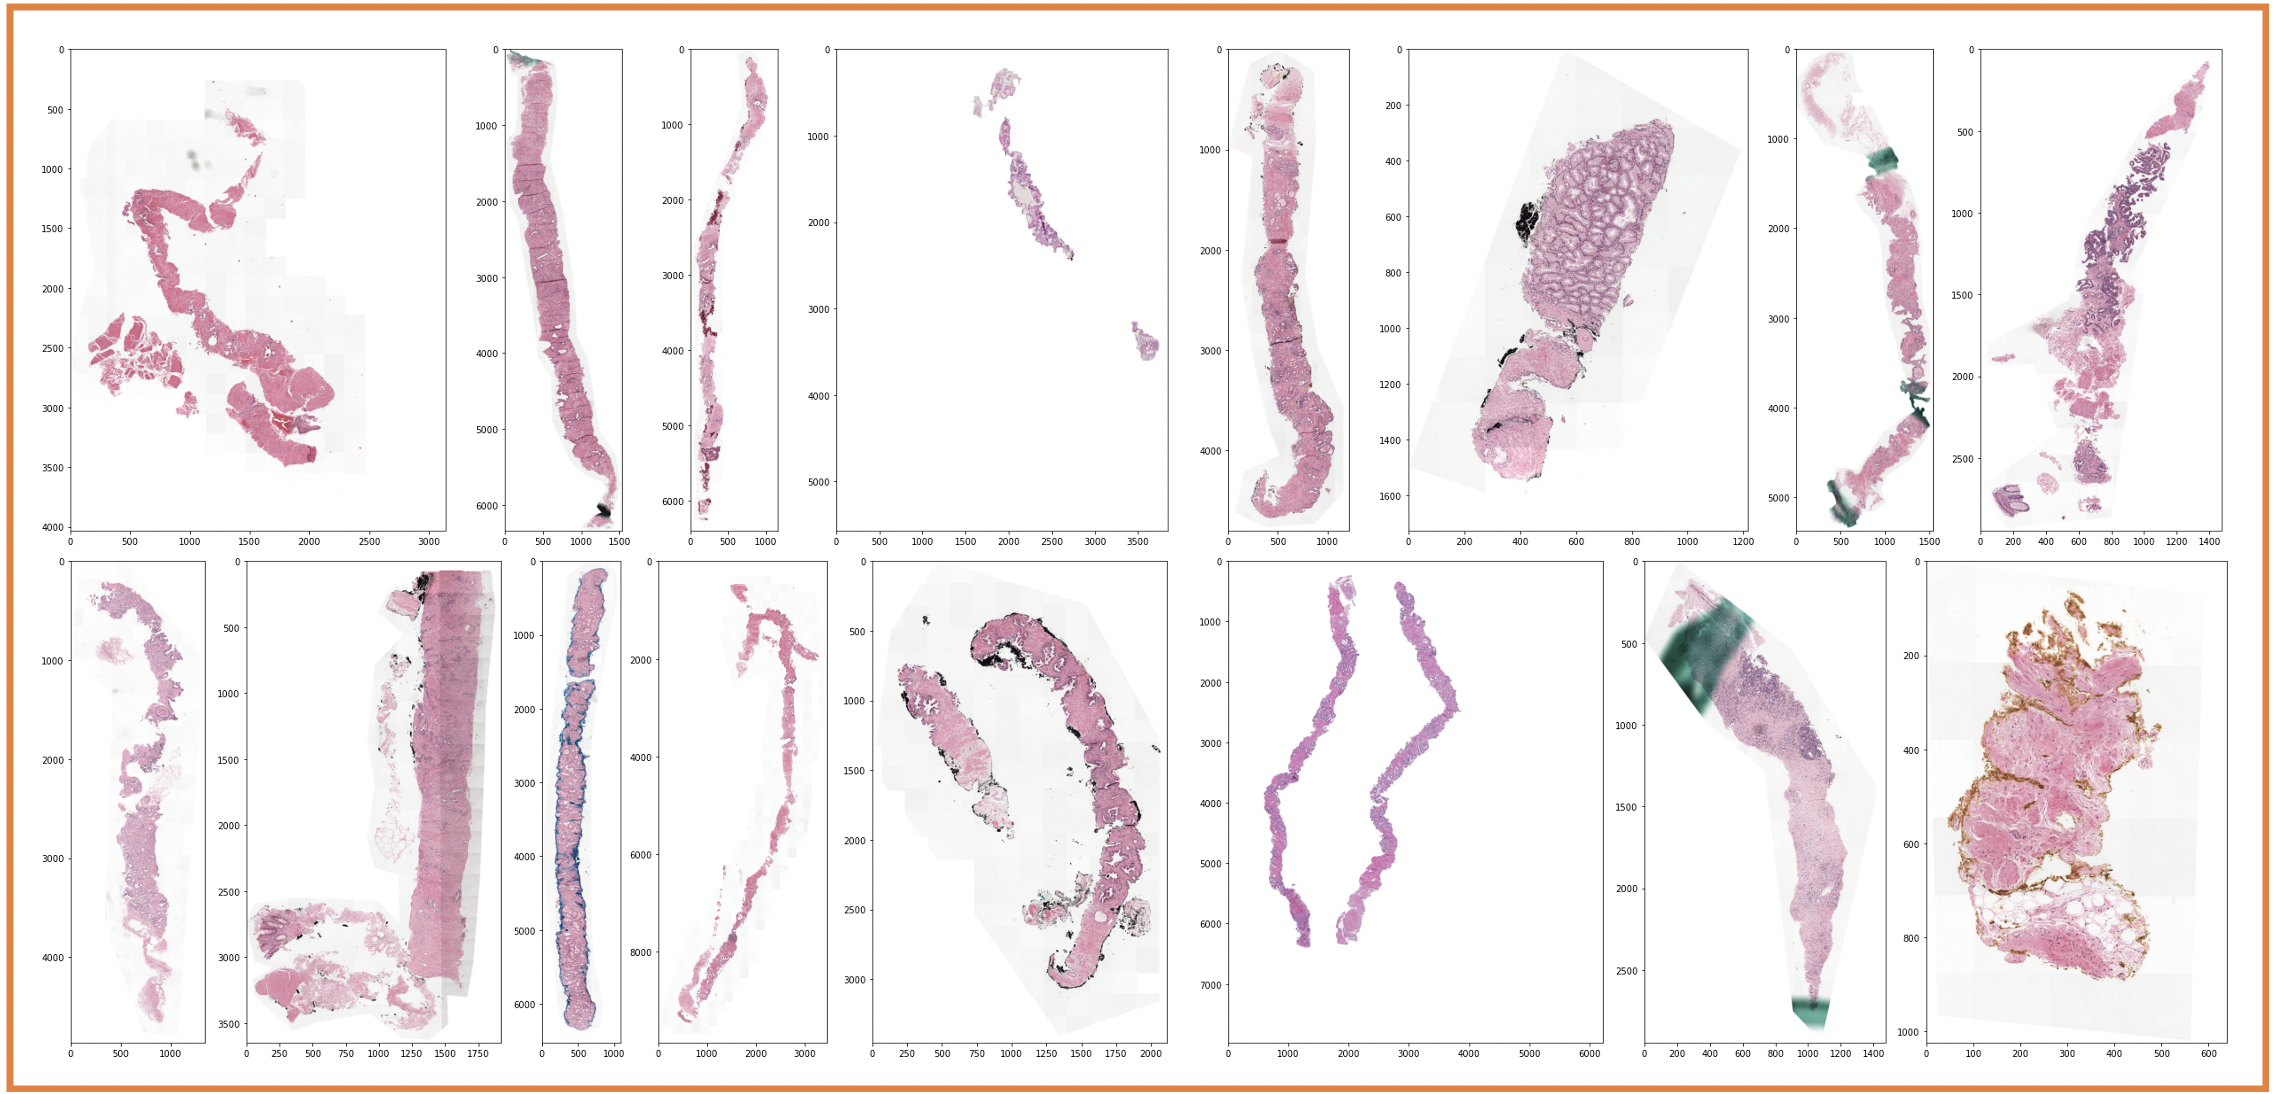
\includegraphics[width=\linewidth]{PANDA.png}
\caption{Sample slides in the public training set of PANDA. We can see WSI have various image quality, including different image size, diverse H\&E stain colors, pen marks, gray background, artifacts, and duplicates}
\label{fig:panda}
\end{figure}


\textbf{PANDA} The dataset of Prostate cANcer graDe Assessment (PANDA) Challenge is the largest multi-center whole-slide images datasets of PCa, consisting of three parts: the public training set, public test set for the public leaderboard, and the private test set for the private leaderboard. Figure \ref{fig:panda} shows sample slides in PANDA,  \par

The public training set contains 10616 H\&E stained WSI which have three magnifications (1x, 4x, 16x) and fours labels: the ISUP grade on a 0-5 scale, the Gleason scores (major \& minor) on a 3-5 scale plus 0 representing non cancer, and label mask. Hidden test sets have roughly 1000 WSI \citep{pandakaggle} and the public test set and private test set are divided by 42\% and 58\% respectively. Table \ref{tab:slides} shows the number of slides in PANDA. Table \ref{tab:distribution} shows the distribution of ISUP grade and Gleason scores in the public training set of PANDA.   \par

\begin{table}[!htb]
\centering
\begin{tabular}{c c c c }
\toprule
Instituation & Public train set & Public test set & Private test set \\
\toprule
Radbound & 5160 & +/- 252 & +/- 348 \\
Karolinska & 5456 & +/- 168 & +/- 232 \\
\textit{Total} & \textit{10616} & \textit{+/- 420} & \textit{+/- 580} \\
\bottomrule
\end{tabular}
\caption{Table 1: Number of slides in PANDA. The proportion of Karolinska in test sets is around 40\%.}
\label{tab:slides}
\end{table}



Both Radboud University Medical Center (Radboud) and Karolinska Institute (Karolinska) contributed the data with different data processing and label methods. 

Slides from Radbound are labeled by students and label masks are annotated by automatic grading system, ranging from 0 to 5. The proportion of noisy labels is around 85\% \citep{wouter_bulten_2020_3715938}.

Slides from Karolinska may have pen marks adjacent to cancer area and are labeled by a single pathologist on Gleason scores which are then converted to ISUP grade. Label masks range from 0 to 2. 

All the private test set and most of public test set are labeled by up to three pathologists on ISUP grade and then get a concensus score and they are free from pen marks.  \par




\begin{table}[!htb]
\centering
\begin{tabular}{c | c | c | c | c | c | c | c | c | c | c | c }
\toprule
ISUP & \multicolumn{1}{c |}{0} & \multicolumn{1}{c |}{1} & \multicolumn{1}{c |}{2} & \multicolumn{1}{c |}{3} & \multicolumn{3}{c | }{4} & \multicolumn{3}{c|}{5} & \multirow{2}{*}{Total} \\
\cline{2-11}
Institutions & 0+0 & 3+3 & 3+4 & 4+3 & 4+4 & 3+5 & 5+3 & 4+5 & 5+4 & 5+5 &  \\
\toprule
Radbond & 967 & 852 & 675 & 925 & 660 & 67 & 41 & 641 & 221 & 111 & 5160 \\
\hline
Karolinska & 1925 & 1814 & 667 & 318 & 466 & 13 & 2 & 208 & 27 & 16 & 5456 \\
\hline
\textit{Total} & \textit{2892} & \textit{2666} &  \textit{1342} & \textit{1243} & \textit{1126} & \textit{80} & \textit{43} & \textit{849} & \textit{248} & \textit{127} & \textit{10616} \\
\bottomrule
\end{tabular}
\caption{Distrubution of ISUP and Gleason scores from two data providers in the public training set in PANDA. The first line is ISUP grades, the second line is Gleason scores under the corresponding ISUP category}
\label{tab:distribution}
\end{table}





\subsection{Metric} We adopted quadratic weighted kappa, which is the PANDA challenge official metric. This metric measures the agreement of two raters, typically varying from 0 (random agreement) to 1(complete agreement) and it can go below 0. \par
The way to calculate quadratic weighted kappa is shown as formula. First, N refers to the number of classes. O, E, w are three N x N matrixes, in which $w_{i,j}$ is calculated based on the difference between actual and predicted values, shown in Equation \ref{equ:w}. Finally, cohen kappa is calculated by the Equation \ref{equ:k}
\begin{equation}
w_{i,j} = \frac{(i-j)^2}{(N-1)^2} \\
\label{equ:w}
\end{equation}
\begin{equation}
k = 1 - \frac{\sum_{i,j}w_{i,j}O_{i,j}}{\sum_{i,j}w_{i,j}E_{i,j}}
\label{equ:k}
\end{equation}




\subsection{Setup}
At first, the overview of the training and prediction pipeline is illustrated in Figure \ref{fig:pipe}. \par

\begin{figure}[!htb]
\centering
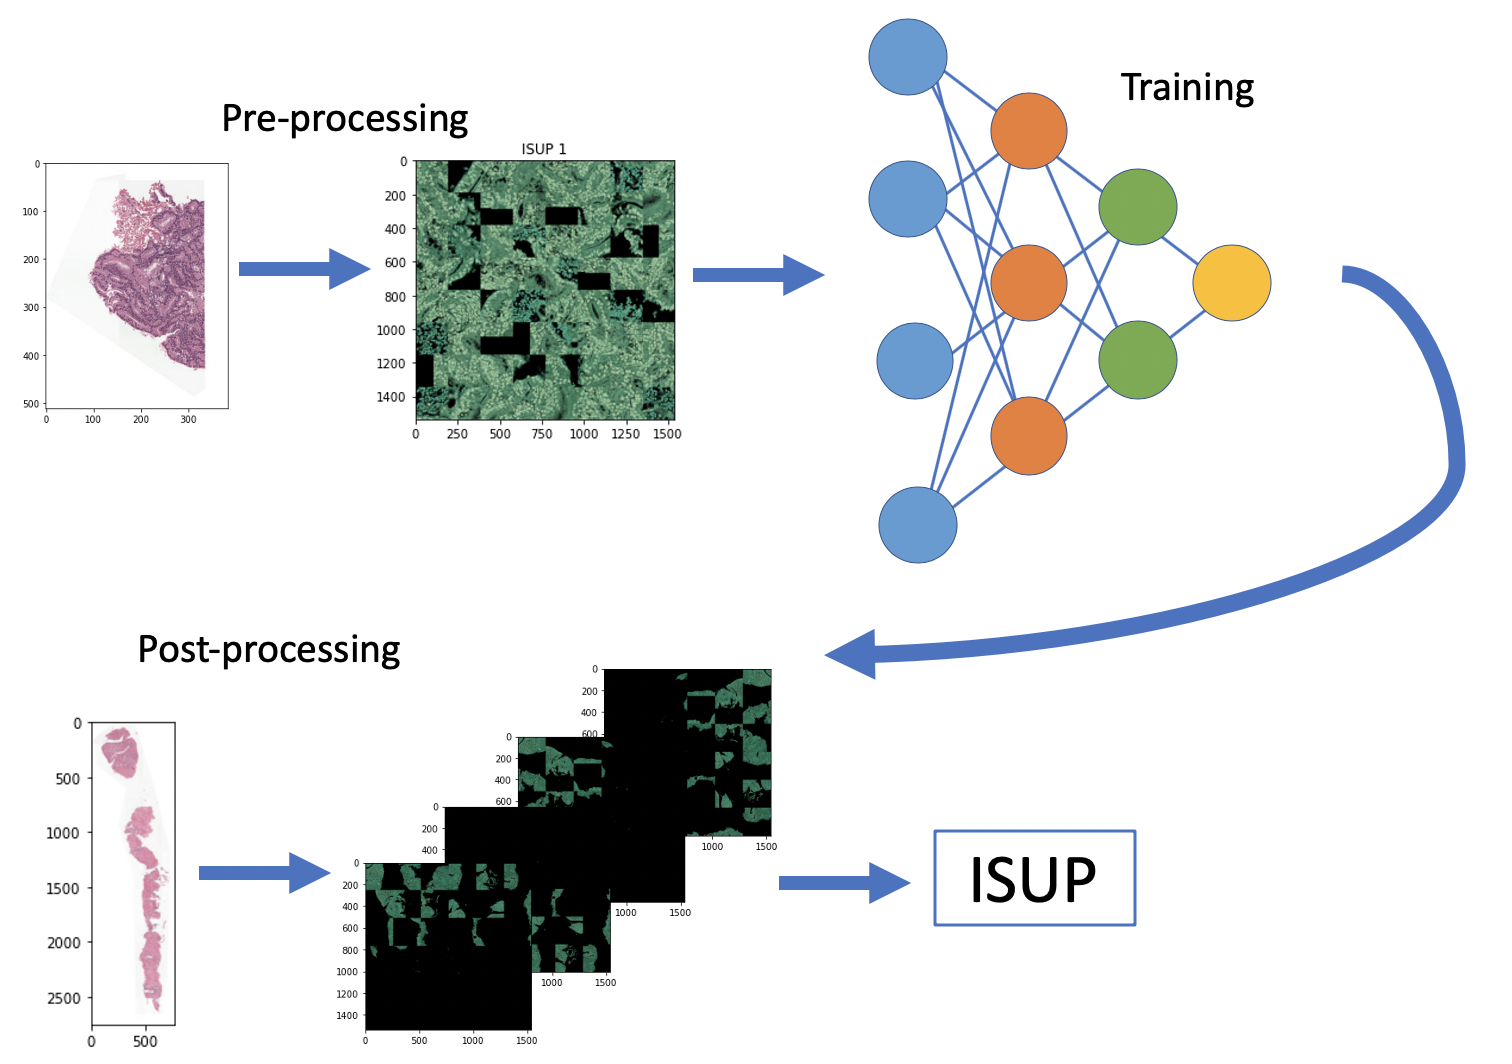
\includegraphics[width=0.6\linewidth]{pipeline.png}
\caption{Overview of overal pipeline}
\label{fig:pipe}
\end{figure}


\textit{Stratified 8 folds split.} The partition of the training and evaluation set is important to the model calibration. In the Deepfake challenge, we used 80\% as the training set and 20\% as the validation set. But this method may cause overfitting in local validation since even planting seed cannot guarantee the code reproducibility and get the same validation set each time. In the PANDA challenge, we used Stratified sampling to split the training data into eight folds and we used the fold 0 (1327 slides) as the hold out set for local validation. Table \ref{tab:split} shows the number of slides in local training and validation. This method proves to be reliable. 

\begin{table}[!htb]
\centering
\begin{tabular}{c | c | c }
Institutions & Training (7/8)  & Evaluation (1/8) \\
\toprule
Radmound &  4517 & 684 \\
Karolinska &  4770 & 643 \\
\textit{Total} & \textit{9289} & \textit{1327} \\
\bottomrule
\end{tabular}
\caption{Number of slides by Stratified 8 fold split}
\label{tab:split}
\end{table}




\textit{Image size.} Image size has influence on model performance. We conducted experiments on 512 and 1536 respectively. Score of image size 512 is up to 0.78 and the score of 1536 would boost to 0.85. We reckon larger image size is better since it can accommodate more information. Besides, the tissue information is very delicate that when compressed into small image size, the difference between Gleason grades would not be evident. We also tried 1024 which can allow us to use bigger batch size but it still shows 1536 is the best image size. For Efficientnet-B4, we used 800. Though we can fit at most 800 as image size but it has no improvement on the performance. We reckon this is because the model size of Efficientnet-B4 is larger, thus 850 would be easier to have overfitting. 

\textit{Batch size.} We used batch size 2 in our experiments, which is the largest we can fit into our 16G memory GPU with image size 1536. We tried to tackle the problem of small batch size by accumulation step, replacing batch normalization with layer normalization and instance normalization. Accumulation step refers to upgrade the gradient by every 4 steps. We found layer normalization damage the model training dramatically, instance normalization damages slightly, and accumulation step has no effect. 

In the aspects of backbone models, we tried Resnet \citep{he2016deep}, Efficientnet-B0, Efficientnet-B1, Efficientnet-B4 \citep{tan2019efficientnet}. We found there is no much difference in model types, but the data preprocessing, training planning, and post processing have huge impacts. Thus, in the later stage of PANDA competition, we focused on Efficientnet-B1 to do experiments. 


\subsection{Data preprocessing}

\textit{Dynamic switch level}. We found the WSI has diverse image size. For example, the image sizes in the middle resolution (4x) range from 1000 to 14000 pixels (Figure \ref{fig:size}). To tackle this problem, we proposed dynamic switch level. When both the image height and width are smaller than 1000 pixels, we would use the highest resolution (16x).


\begin{figure}[!htb]
\centering
\minipage{0.59\textwidth}
	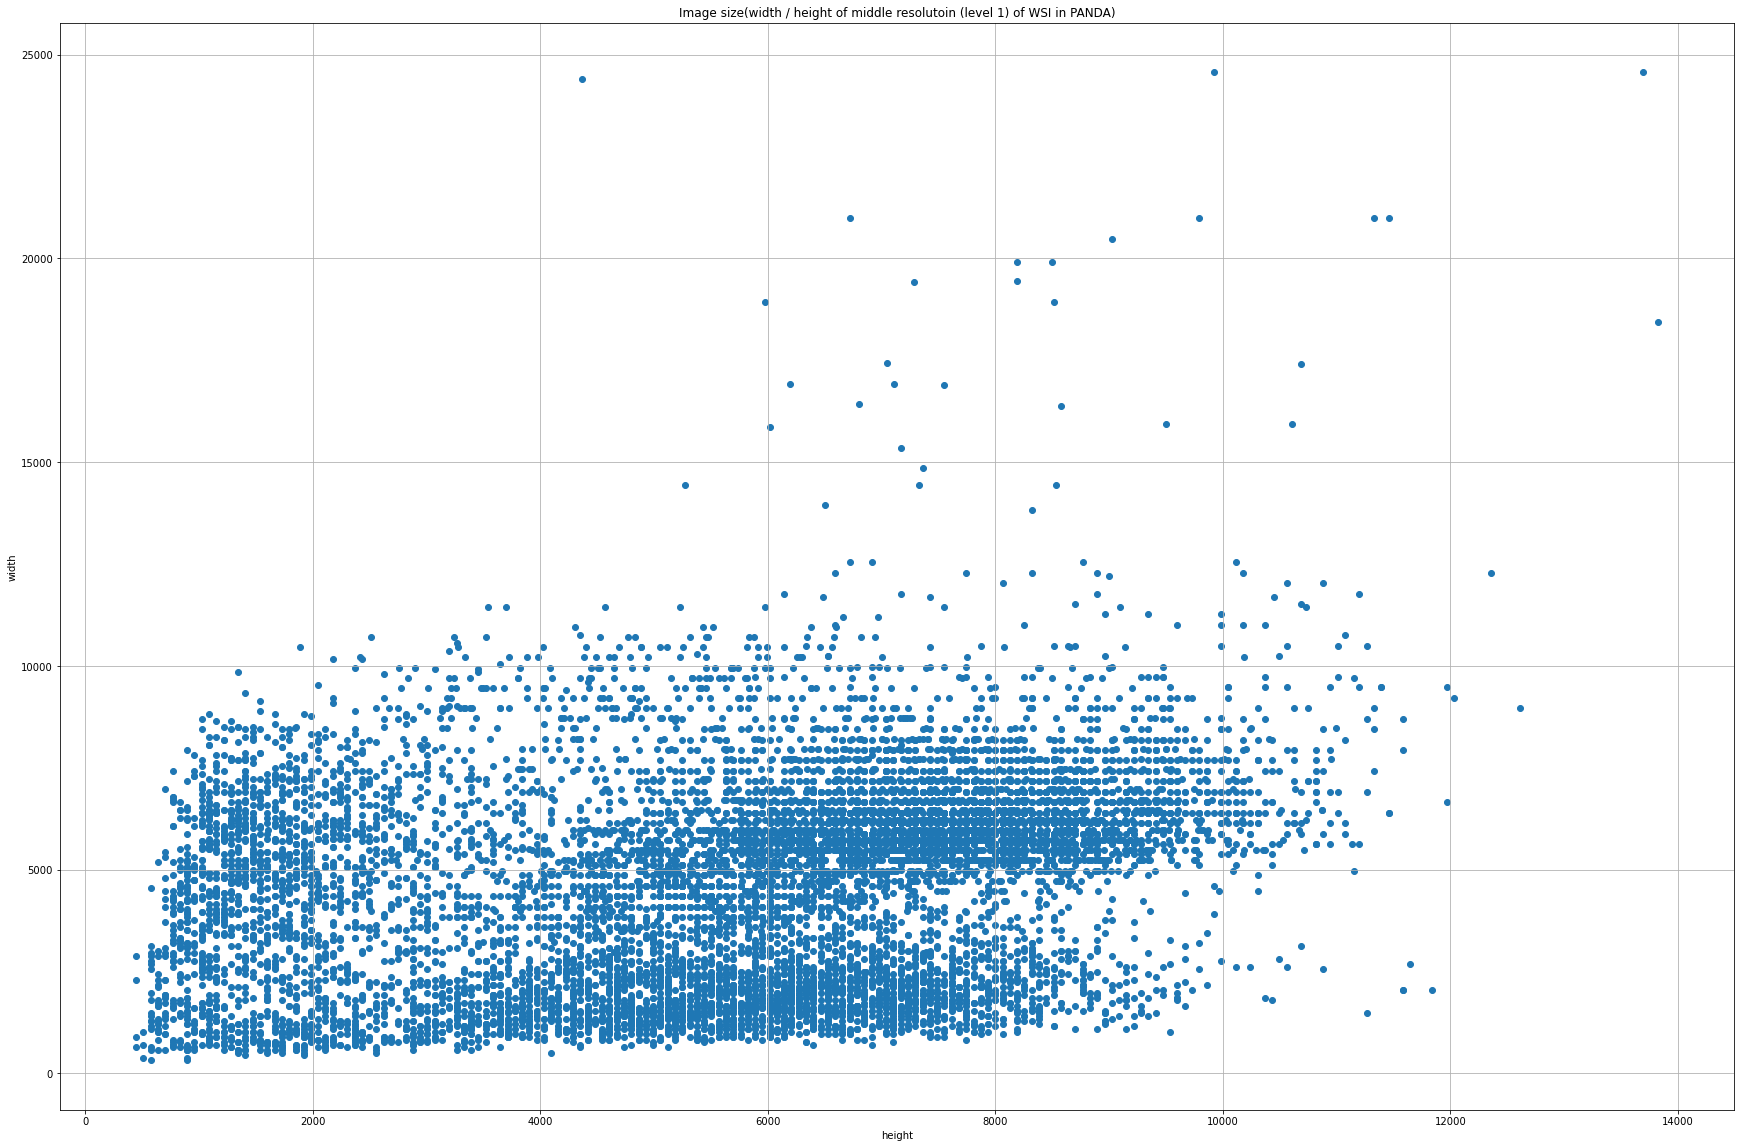
\includegraphics[width=\linewidth]{panda-level1-img-size.png}
	\caption{Dramatically various image size of middle resolution (level 1, 4x) of WSI in PANDA}
	\label{fig:size}
\endminipage\hfill
\minipage{0.38\textwidth}
	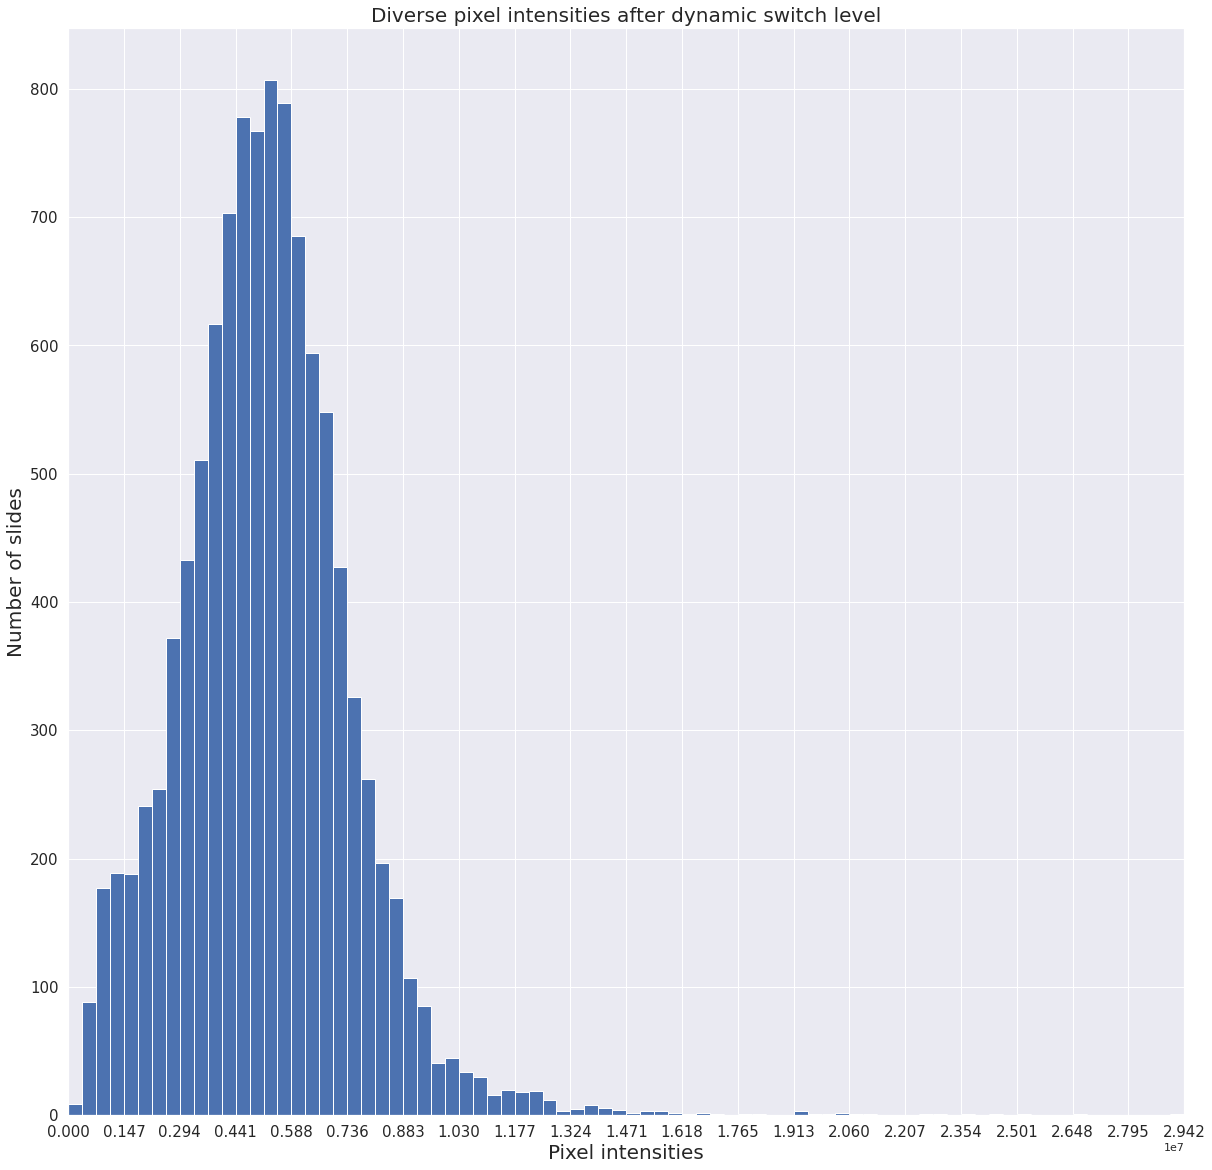
\includegraphics[width=\linewidth]{pixel-intensities.png}
  	\caption{Diverse pixel intensities after dynamic switch level}
	\label{fig:pixel}
\endminipage\hfill
\end{figure}



\textit{Bin threshold}. Foreground extraction is one common step to remove non-tissue backgrounds in WSI preprocessing \citep{duran2020prometeo}. We proposed bin threshold which is very simple and fast. When the pixel value is bigger than a specific value, the pixel would be white. We experimented that 235 is a good threshold which can filter out gray areas and keep the tissue maximally. Though very simple to implement, it has super fast speed and good impact on model performance compared with other thresholds. For example, we tried Otsu threshold \citep{otsu1979threshold} to do foreground extraction. Though the slides filterd by Otsu threshold have beautiful visual result, the model performance is not good.

We also tried color filters (red, blue, green) to filter out pen marks accordingly. In training, we didn't use red color filter since red is very close to the color of H\&E stained slides. It is very easy for the red color filter to remove too much information.  When using green and blue color filters, we found the training speed doubled but the model performance was not good. So we didn't use color filters. 


\textit{Dynamic tiling}. Feeding whole WSI into model is impossible and inefficient since our GPU memory (16G) doesn't support the large image size of WSI. Even resizing WSI is not a good way because there are many white backgrounds which makes the model training very inefficient. Turning the research of interest (ROI) of WSI into patches is a common method to preprocess WSI \citep{li2018path}. However, the provided WSI has diverse pixel intensities. Figure \ref{fig:pixel} shows the pixel numbers of WSI generally range from 735000 to 29420000 after dynamic switch level and bin threshold. Unified tiling method such as sampling 36 patches with patch size 256 (256X256X36) would cause this dilemma: for slides with small pixel intensity, there are too many blank tiles while for slides with huge pixel intensity, 36 patch number is not enough. Therefore, we propose dynamic tilling which maximally get keep the information of ROI. 

Dynamic tiling is implemented as follows: at first, we start from 256X256X36. We have a threshold called WHITE\_TR to filter out white tiles. WHITE\_TR decides how many proportion of while area takes in a patch will make the patch white tile and be discarded. Some tiles have very little information. We tested that 0.95 for WHITE\_TR is a good threshold. 


\textit{Augmentations.} We applied two levels of data augmentations. On both tile and concatenated image level, we used horizontal flip, vertical flip, and transpose to augment the images. 


\textit{Normalization.} We simply normalized the data with mean 0.5 and standard deviation 0.5. The equation is $X_{i\_normalized} = \frac{X_i - 0.5}{0.5}$, in which $X_i$ is a concated image. We tried to stastically get the mean and standard deviation of the extracted tiles. But since the tiling strategy would change at times to feed different feature distributions to the model, counting mean and standard deviation each time would be time-consuming and meaningless. The influence of these two values have no much difference, thus, we simply use 0.5 for both mean and standard deviation to normalize the data into space of $[-1, 1]$.

The whole data preprocessing pipeline is illustrated in Figure \ref{fig:pre}. The general workflow is as follows: 1) dynamic switch level, 2) bin threshold, 3) dynamic tiling, 4) shuffle tiles, 5) tile level augmentation, 6) concatenated tiles into one image, 7) color reverse and resize image to 1536, 8) image level augmentations and normalization.



\begin{figure}[!htb]
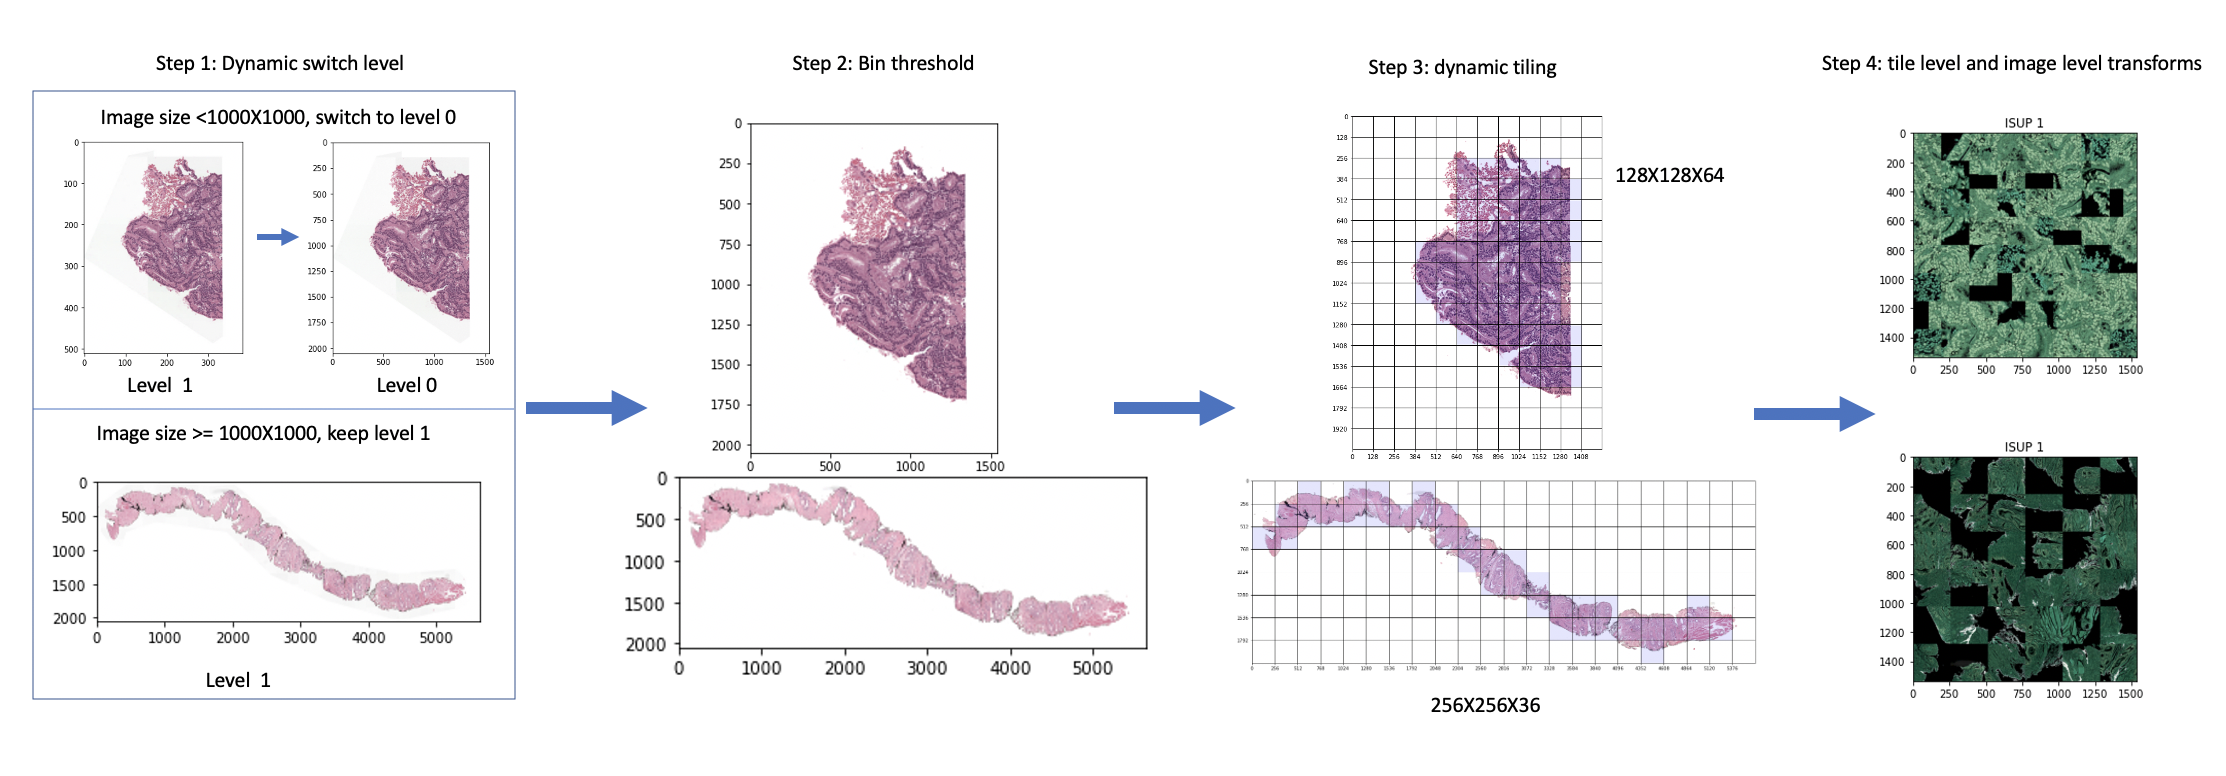
\includegraphics[width=\linewidth]{preprocess-pipeline.png}
\caption{Overview of dynamic data preprocessing pipeline}
\label{fig:pre}
\end{figure}


\subsection{Training}

\textit{Efficientnet} \citep{tan2019efficientnet} was designed by NAS \citep{liu2018darts} and has proved to be successful in many applications. Thus, we use Efficientnet as base architecture. We used Efficientnet-B0, Efficientnet-B1, and Efficientnet-B4.

\textit{Adam} \citep{kingma2014adam} was used with learning rate 0.001. We run one epoch on the freezed model to find suitable learning rate, we found 0.001 is a suitable learning rate. We used Imagenet pretrained weights. All the experiments were conducted on Kaggle GPU and Google Cloud Project (GCP). 

\textit{Head and loss.} We only used single head to predict ISUP score. We tried using multi-heads to predict ISUP, Gleason major, and Gleason minor simultaneously but found no improvement. We use mean squared error (MSE) as loss function and regression. The formula of MSE is shown in Equation \ref{equ:mse}.
\begin{equation}
MSE = \frac{\sum_{i=1}^n(y_i - y_i^p)^2}{n}
\label{equ:mse}
\end{equation}





\textit{Stage training.} In PANDA challenge, we utilized a dynamic training strategy called stage training.We divide the whole butch training into 3 stages: debug, warmup, and cover stages. In debug training, only a small amount of training data is used to detect model effectiveness. In warmup training, 1/3 of training data is used to warm up the model. We found this method is better than normal butch training. Finally, we used whole training data to do cover training, which aims to cover all the feature space in the training space. 

\textit{Training speed boost.} We used some approaches to boost the training speed and can reduce about 30 minutes in one epoch. Early parts including disk I/O and data preprocessing in training are usually the bottleneck of training speed since they cannot be benefited from accelerators such as GPU and TPU. We tried to reduce the process of data preprocessing as much as possible by extracting tiles (stop at step 3 in Figure \ref{fig:pre}) or premade the training dataset completely offline (stop at step 4 in Figure\ref{fig:pre}). The former allows us to do shuffle and augmentations and the later has a faster speed.  \par
In addition, we used fp16 which allows the model to calculate faster with shorter precision \citep{haidar2018harnessing}. We also tried to replace Swish activation \citep{ramachandran2017swish} in Efficientnet with Hard-Swish \citep{howard2019searching} which uses linearity to approximate the curve of sigmoid. We also tried using TPU accelerator that we converted the premade training dataset into tfrecords format and we need to convert our codes from Pytorch to Tensorflow since Tensorflow is better compatible to TPU. But at that time we were close to the PANDA competition deadline and this would shift our energy to code migration, thus, we didn't implement this method in the end. 



\textit{Oversampling and noisy label.} During training, we found some interesting phenomenons. The local validation score would reach a plateau round 0.85 and fluctuate while the training score can keep going up. If we continue training, there will have overfitting. We suspect this is caused by noise labels. In addition, we found that in local validation, the set got wrong predictions almost keeps same. To deal with these problems, for slides with small training errors, we utilized oversampling, training them for extra 10 times while for slides with huge training errors, we regarded them as noisy labels and discarded them.


\subsection{Post processing}

Post processing is significant to boost the model performance. Our Effiicentnet-B1 achieved public leaderboard score (public LB)  0.85 and 0.87261, without and with post processing respectively. We explored further after the PANDA competition and can get 0.88179 for the same model. The boost space is around 0.3. 

There is a bit difference between preprocessing and post-processing pipelines. For tiling, we found 256X256X36 is better. In addition, we flipped the concatenated image three times (vertical flip, transpose, and vertical flip + transpose). Namely, our prediction for one slide is the mean of 4 predictions (original image + 3 flips). This can boost public LB from 0.85 to 0.86. We also tried 8 flips (4flips + 4 horizontal flips) but it only doubles the prediction time with no improvement. 

In the final prediction, we used dynamic switch level (pop1), bin threshold (pop2). We also cropped the image(pop3) and transposed the image(pop4) when the height is smaller than width. This achieved public LB 0.87261 and private LB 0.92096.  

\begin{table}[!htb]
\centering
\begin{tabular}{c | c | c | c | c}
\toprule
Stage & Name & local predict cohen & public LB & private LB \\
\toprule
pop1 & without switch level & 0.8458 & 0.86786 & \textbf{0.92438} \\
pop1 & \textbf{switch level} & 0.8458 & \textbf{0.87261} & 0.92096 \\
\hline
pop2 & without foreground threshold & 0.7922 & 0.85219 & 0.87583 \\
pop2 & \textbf{bin threshold (235)} & 0.8458 & \textbf{0.87261} & \textbf{0.92096} \\
pop2 & Otsu threshold & 0.9221 & 0.87014 & 0.91954 \\
\hline
pop3 & \textbf{without crop} & 0.9267 & \textbf{0.88116} & 0.91598\\
pop3 & crop  & 0.8458 & 0.87261 & 0.92096 \\
pop3 & without crop + mode 0 \& 2 & 0.9235 & 0.87761 & \textbf{0.92393} \\
\hline
pop4 & \textbf{without transpose} & 0.8548 & \textbf{0.87422} & \textbf{0.92458} \\
pop4 & transpose  & 0.8458 & 0.87261 & 0.92096 \\
\hline
pop & highest public LB  & 0.9267 & \textbf{0.88179} & 0.91777 \\
\bottomrule
\end{tabular}
\caption{Post-processing pipeline comparison}
\label{tab:pos}
\end{table}


After competition, we want to validate if each step is valid. Table \ref{tab:pos} confirmed that dynamic switch level and bin threshold are effective and we can remove cropping and transpose to get higher public LB (0.88179). Here, I use the public LB rather than private LB to evaluate performance since only public LB is accessible to competitors during the competition. Public LB is for competitors to check their model performance, but private LB is to evaluate model generalization.


Table \ref{tab:com} shows our post processing method is effective. Even removing cropping and transpose, the private LB decreased a bit, the score still ranks 91 out of 1010 teams. 

We also tried ensemble and cross validation but they have no effect in our experiments.

\begin{table}
\centering
\begin{tabular}{c | c | c | c}
\toprule
Stage & public LB & private LB & Rank (out of 1010 teams) \\
\toprule
Without post-processing & 0.85830 & 0.89123 & - \\
\hline
Add 4 flips & 0.86349 & 0.89074  &  - \\
With post-processing & 0.87261 & 0.92096 & 50 \\
\hline
Remove cropping and transpose & 0.88179 & 0.91777 & 91 \\
\bottomrule
\end{tabular}
\caption{Comparison between without and with post-processing}
\label{tab:com}
\end{table}



\section{Results}

We tested our method on the PANDA challenge on Kaggle as edu3d.co team. The intention of this competition is to develop a generalized automated grading algorithm which can apply in multi-center dataset. The evaluation datasets are composed of the public test set and the private test set. Both are not disclosed to the public. We achieved private LB 0.920096, which can rank 50 out of 1010 teams according to the finalized private learderboard. The submission for PANDA challenge remains open to be the benchmark for prostate cancer automated diagnosis. 






\section{Conclusion}

Our method dynamic training planning (dynamic data preprocessing, training planning, and post processing) explores the potential of existing models, which has significant meaning since one significant aspect of Kaggle competition is feature engineering. From past Kaggle competitions, all of Resnet, Densenet, or Efficientnet has been used by the first winner. How to maximally extract features from available training set and map them to the unseen test set is one of the biggest challenges for researchers to solve. In the end, our solutions still have much space to explore.. 

 

\subsubsection*{Acknowledgments}

I would like to thank my supervisor Professor Ramesh Sankaranarayana for his instruction.



\bibliographystyle{agsm}
\bibliography{ref}

\end{document}
